\documentclass{tufte-book}
%\documentclass[letterpaper]{scrbook}
\hypersetup{colorlinks}
\usepackage{amsmath, amsthm, amssymb}
\usepackage{pgfplots}
\usepackage{mathpazo}
\usepackage[T1]{fontenc}
\usepackage[protrusion=true,expansion=true]{microtype}
\usepackage{marvosym}
\usepackage{mathrsfs}
\usepackage[all]{xy}
\usepackage{enumerate}
\usepackage{booktabs}
\usepackage{xspace}
\usepackage{dialogue}
\usepackage{sectsty}
\allsectionsfont{\sffamily}
\usepackage{cleveref}
%\usepackage{exercise}
%\usepackage[pagebackref,colorlinks]{hyperref}

\usepackage{proofspreamble}

\setcounter{tocdepth}{1}
\setcounter{secnumdepth}{3}
\titleformat{\chapter}
  [block]% shape
  {\relax\ifthenelse{\NOT\boolean{@tufte@symmetric}}{\begin{fullwidth}}{}}% format applied to label+text
  {\itshape\huge\thechapter}% label
  {1em}% horizontal separation between label and title body
  {\huge\rmfamily\itshape}% before the title body
  [\ifthenelse{\NOT\boolean{@tufte@symmetric}}{\end{fullwidth}}{}]% after the title body

\title{On Writing Proofs}
\author{Shahed Sharif}

\begin{document}

\maketitle

\tableofcontents

\chapter{Propositional Logic}
\label{cha:propositional-logic}

\section{\Knights and \knaves}
\label{sec:knights-knaves}

A certain island in the middle of the Pacific Ocean is inhabited by two types of people, known as \knights and \knaves. It is known that \knights always make true statements, while \knaves always lie. One day, you visit the island and encounter three of the inhabitants: Azog, Bartholomew, and Cynthia. You ask Azog whether he is a \knight or a \knave. The following conversation ensues:

\begin{example}\label{ex:knight-knave-1}
  \begin{dialogue}
    \speak{Azog} [mumbles inaudibly]\sidenote{Both \knights and \knaves are known to mumble occasionally!}
    \speak{You} What did you say?
    \speak{Bartholomew} He said that he's a \knave. 
    \speak{Cynthia} Bartholomew lies!
  \end{dialogue}
\end{example}

The question is, who is a \knight and who is a \knave? Take a moment to solve this problem.

\begin{center}
{\Large\Clocklogo}
\end{center}

The next few sections contain problems of this sort; that is, a number of inhabitants make a number of statements, and based on these statements, you must deduce something, usually who is a \knight and who is a \knave. There is always a straightforward way of approaching these problems: try every possibility! In the above example, Azog can be a \knight or a \knave, Bartholomew can be a \knight or a \knave, and Cynthia can be a \knight or a \knave, giving $2 \cdot 2 \cdot 2 = 8$ possibilities total.\sidenote{A common error is to think that there are 6 possibilities total. If you thought so, then you should list them all out.} Most of these possibilities will make no sense, as you'd end up having a \knight making a false statement or a \knave making a true statement. As a simple example, consider the puzzle

\begin{dialogue}
  \speak{Avery} Two plus two is five.
  \speak{Belvedere} The sky is blue.
\end{dialogue}

Since there are two people in the problem, there are $2 \cdot 2 = 4$ potential solutions: \marginnote{Trying out every single option is known as the \emph{brute force} approach, and as you can see from this last example, one should only use it as a last resort. Instead, make key observations to shorten your work.}  Avery is a \knight and Belvedere is a \knight, Avery is a \knight and Belvedere is a \knave, Avery is a \knave and Belvedere is a \knight, or Avery is a \knave and Belvedere is a \knave. But clearly testing all 4 possibilities is a very slow way of solving the problem! 

Now let's do \Cref{ex:knight-knave-1}.
\begin{claim}
  Bartholomew is a \knave and Cynthia is a \knight. Azog's type cannot be determined.
\end{claim}

\begin{proof}
  If Azog were a \knight, then he could not say that he is a \knave, for then he'd be lying. If Azog were a \knave, then again he could not say that he is a \knave, for then he'd be telling the truth. Either way, Azog cannot have said that he is a \knave. Therefore Bartholomew's statement is false, \marginnote{Note that Bartholomew isn't saying that Azog is a \knave, but rather that \emph{Azog says} that Azog is a \knave.} hence Bartholomew is a \knave, and Cynthia's statement is true, hence she is a \knight. As for Azog, from the information given, there is no way of determining what he is.
\end{proof}


Notice how we wrote this out: first, the answer under the label ``Claim'', then the explanation with the label ``Proof''. The end of the proof is marked with a box, called a \emph{tombstone}.\sidenote{Because you totally killed the problem.} Proofs are the main subject of this book. You'll notice immediately that the proof is written in complete sentences put together into a paragraph; that is, a proof is a written form, like an essay, and should conform to the usual standards for a properly written essay, including correct spelling and grammar.\marginnote{There are many ingredients to a correctly written mathematical proof. We will discuss these ingredients in detail in the remainder of this book.} Additionally, the proof is written as a formal, logical argument, where each statement is carefully explained. In the problems below, you should write out your answers in the same format as I've done above.

%%% Local Variables:
%%% TeX-master: "Proofs"
%%% End:
\probsec{~\ref{sec:knights-knaves}}

  In all of the following, named characters are \knights or \knaves.\marginnote{Remember that all answers should be explained in complete sentences! The goal is clarity.}

\begin{enumerate}
    \item Suppose Adonis says, ``I am a \knight.'' What can you conclude?

    \item Suppose you encounter Ariadne and Bilal.
  \begin{dialogue}
    \speak{Ariadne} Bilal would say that I am a \knight.
    \speak{Bilal} That's not true.
  \end{dialogue}
  What can you conclude?

    \item You meet Alivia and Boris.
  \begin{dialogue}
    \speak{Alivia} Boris would say that I am a \knave.
    \speak{Boris} Alivia would say that I am a \knight.
  \end{dialogue}
  What can you conclude?

    \item You encounter Ayumi, Bethesda, and Coco.
  \begin{dialogue}
    \speak{Ayumi} Bethesda would say that Coco is a \knave.
    \speak{Bethesda} Coco would say that Ayumi is a \knave.
    \speak{Coco} Ayumi is a \knight.
  \end{dialogue} 
  You additionally know that at least one of the three is a \knight. What can you conclude?

  \item You encounter Aragorn, Boromir, and Celeborn.
  \begin{dialogue}
    \speak{Aragorn} Boromir would say that Celeborn is a \knave.
    \speak{Boromir} Aragorn is a \knave.
    \speak{Celeborn} Boromir would say that I am a \knave.
  \end{dialogue}
  What can you conclude?
\end{enumerate}



\section{Conjunctions}
\label{sec:conjunctions}

Suppose Arjun makes the following statement:
\begin{example}
  \begin{dialogue}
    \speak{Arjun} I am a \knave and Bathsheba is a \knight.
  \end{dialogue}
\end{example}

What are Arjun and Bathsheba? This statement is an example of the conjunction AND. In order for the statement to be true, both parts must be true; to be false, \emph{at least one part} must be false. That means the first part is false, or the second part is false, or both are false. Consider the following examples:
\begin{enumerate}
    \item The sky is blue and $2 + 2 = 4$.
    \item The sky is green and $2 + 2 = 4$.
    \item The sky is blue and $2 + 2 = 5$.
    \item The sky is green and $2 + 2 = 5$.
\end{enumerate}
Of these, the first is true, and the rest are false.

Now we solve the problem.
\begin{claim}
  Arjun and Bathsheba are both \knaves.
\end{claim}

\begin{proof}
  Suppose Arjun is a \knight. Then both parts of his statement are true. But the first part of his statement is that he is a \knave, which is the opposite of what we assumed. So Arjun must be a \knave. Thus his statement as a whole must be false. The first part of his statement, that he is a \knave, is true, so the second part must be false. Therefore Bathsheba is also a \knave.
\end{proof}

Notice that making two separate statements is not the same as putting an AND between them; that is, if the puzzle were instead
\begin{example}
  \begin{dialogue}
    \speak{Arjun} I am a \knave. Bathsheba is a \knight.
  \end{dialogue}
\end{example}
then you'd have to say, ``That's impossible!'' Why? Because Arjun could never make the statement ``I am a \knave.''

Try this puzzle:
\begin{example}
  \begin{dialogue}
    \speak{Annalee} Either I am \knave or Bijou is a \knight.
  \end{dialogue}
\end{example}
What are Annalee and Bijou? Here we have a different type of conjunction: OR. The or in mathematics functions slightly differently than in conversational English in that it is true if one \emph{or both} of the parts are true.\marginnote{If we want one thing to be true but not both, we'd say so explicitly: ``I am tall or I am shy, but not both.'' This is sometimes called \emph{exclusive or}. Regular or is \emph{inclusive}.} Consider the following statements:
\begin{enumerate}
    \item The sky is blue or $2 + 2 = 4$.
    \item The sky is green or $2 + 2 = 4$.
    \item The sky is blue or $2 + 2 = 5$.
    \item The sky is green or $2 + 2 = 5$.
\end{enumerate}
The first three are true, while the last one is false. \marginnote{There is a well-known joke about a logician and his wife. The wife has just given birth, and asks her husband, ``Is it a boy or a girl?'' to which he responds, ``Yes.''}

\begin{claim}
  Both Annalee and Bijou are \knights.
\end{claim}

\begin{proof}
  If Annalee is a \knave, then the first part of her statement is true, which is impossible. Therefore Annalee is a \knight. Since now the first part of her statement is false, the second part must be true. Therefore Bijou is a \knight as well.
\end{proof}

%%% Local Variables:
%%% TeX-master: "Proofs"
%%% End:
\probsec{~\ref{sec:conjunctions}}
\begin{enumerate}
    \item You meet Allen, Burroughs, and Corso.
  \begin{dialogue}
    \speak{Allen} Burroughs and Corso are \knights.
    \speak{Burroughs} Either I or Allen is a \knave.
  \end{dialogue}
  What can you conclude?

    \item You meet Anand, Botvinnik, and Capablanca.
  \begin{dialogue}
    \speak{Anand} Either Botvinnik is a \knave or Capablanca is a \knight.
    \speak{Botvinnik} Capablanca and I are both \knaves.
  \end{dialogue}
  What can you conclude?

    \item You encounter Asia, Brussels, and Cuba.
  \begin{dialogue}
    \speak{Asia} Cuba and I are both \knights.
    \speak{Brussels} Either Asia or Cuba is a \knave.
    \speak{Cuba} Asia and Brussels are both \knaves.
  \end{dialogue}
  What can you conclude?

    \item You encounter Al, Bonnie, Clyde, and Dillinger. One of them is a \knave who stole a very valuable mathematical manuscript. Determine from their statements who is the thief.
  \begin{dialogue}
    \speak{Al} Dillinger is the thief.
    \speak{Bonnie} At least one of us is a \knight.
    \speak{Clyde} At least one of us is a \knave.
    \speak{Dillinger} Both Bonnie and Clyde are \knights.
  \end{dialogue}

    \item You meet Arkana, Bullard, Robin, and Corinthian.
  \begin{dialogue}
    \speak{Arkana} Either Bullard is a \knight or Robin is a \knave.
    \speak{Bullard} Either Arkana or Corinthian is a \knave.
    \speak{Robin} At least one of the other three is a \knave.
  \end{dialogue}
  What can you conclude?

    \item You run into Agamemnon, Briseis, Cassandra, and Diomedes.
  \begin{dialogue}
    \speak{Agamemnon} Briseis is a \knight and Cassandra is a \knave.
    \speak{Briseis} Cassandra is a \knave and Diomedes is a \knave.
    \speak{Cassandra} Either Agamemnon or Briseis is a \knave.
    \speak{Diomedes} Cassandra is a \knave or Agamemnon is a \knight.
  \end{dialogue}
  What can you conclude?


\end{enumerate}


\section{Conditionals}
\label{sec:conditionals}

A conditional is an \emph{if-then} statement, such as \marginnote{Mathematics essentially consists of a collection of true conditionals.}
\begin{itemize}
    \item If it is raining, then the grass is wet.
    \item If the shape is a square, then it is a rectangle.
    \item If I sleep poorly, then I am tired in the morning.
    \item If $n$ is an even prime, then $n = 2$.
    \item If you have great power, then you have great responsibility.
\end{itemize}
Grammatically, conditionals can be phrased in multiple ways:
\begin{itemize}
    \item The grass is wet whenever it rains.
    \item Every square is a rectangle.
    \item I feel tired every time I sleep poorly.
    \item The only even prime is 2.
    \item Suppose you have great power. Then you also have great responsibility.
\end{itemize}

We consider the following situation:
\begin{example}
  \begin{dialogue}
    \speak{Ashika} If I am a \knight, then Burt is a \knave.
  \end{dialogue}
\end{example}
What are Ashika and Burt?

Dealing with conditionals is considerable trickier than dealing with conjunctions. The general conditional is in the form ``If P then Q,'' where the P and Q stand for statements. In the above example, P is ``Ashika is a \knight'' and Q is ``Burt is a \knave.'' The question is, what does it mean if the conditional is true? And what does it mean if the conditional is false? We demonstrate with a couple easier examples.

\begin{example}
  You are a bouncer at a bar. It is your job to make sure no one underaged is drinking. You see four people at the bar:
  \begin{itemize}
      \item an elderly man drinking water,
      \item an elderly woman drinking scotch,
      \item a young man drinking beer, and
      \item a young woman drinking soda.
  \end{itemize}
  Whose identification do you check?\sidenote{You could of course just check everyone's ID, but generally you want to check the fewest number of people as possible.}
\end{example}

Try this now. The words printed below will wait patiently.

\begin{center}
{\Large\Clocklogo}
\end{center}

Okay, ready? This should be easy: just check the third person's ID. Here, you are checking that the rule
\begin{quote}
  If you are under 21, then your drink must be nonalcoholic.
\end{quote}
is satisfied. There is only \emph{one} situation which breaks this rule: someone under 21 who is drinking an alcoholic beverage. 

Going back to the general case, this implies that the statement ``If P then Q'' is false when both P is true and Q is false, but is otherwise a true statement!

To illustrate this last observation, we consider the following statements:
\begin{enumerate}
    \item If $2 + 2 = 4$, then the sky is blue.\marginnote{One thing to observe about these examples is that in terms of logic, there's no need for there to be a \emph{causal relationship} between the two parts of a conditional. That is, even though there's absolutely no reason in the world that the incorrect arithmetic statement $2 + 2 = 5$ should affect the color of the sky, the statement ``If $2 + 2 = 5$, then the sky is blue'' is still considered true.}
    \item If $2 + 2 = 5$, then the sky is blue.
    \item If $2 + 2 = 5$, then the sky is green.
    \item If $2 + 2 = 4$, then the sky is green.
\end{enumerate}
Of these, the first three are true, and the last is false.
\begin{example}
  Given the statement, ``If it is raining, then the grass is wet'', what would have to be happening right now for the statement to be false? List all possibilities which make the statement false.
\end{example}

% We still haven't talked about the card problem. \marginnote{You should have tried to solve it before you got to this point. If you didn't, you're a lazy bum.}

% \begin{claim}
%   You would turn over the cards labeled A and 7.
% \end{claim}

% \begin{proof}
%   As stated earlier, ``If P then Q'' is true \emph{unless} P is true and Q is false. In this case, P is ``the letter is a vowel'' and Q is ``the number on the other side is even''. For the card labeled N, P is false, so the conditional is automatically satisfied\sidenote{We say a statement or condition is \emph{satisfied} if it is true in that particular case. The statement is true if it is satisfied in all cases.}, and we don't need to turn the card over. For the card labeled 4, Q is true, so again the conditional is also automatically satisfied; we need not turn this card over.

%   For the card labeled A, if the opposite side has an odd number, then the conditional is false; if the opposite side has an even number, then the conditional is true. Thus we need to check the A. The last case is 7. If the opposite side is a consonant, then there is no problem---the conditional is satisfied.\marginnote{If this seems strange, consider the case where opposite the 7 is an E, and opposite the 4 is a C. What does each card tell you about the truth of the conditional?} But if the opposite side is a vowel, then the conditional is false.
% \end{proof}

Now we are ready to do the \knights and \knaves puzzle at the start of this section! We restate it here to refresh your memory:
  \begin{dialogue}
    \speak{Ashika} If I am a \knight, then Burt is a \knave.
  \end{dialogue}

  \begin{claim}
    Ashika is a \knight and Burt is a \knave.
  \end{claim}

  \begin{proof}
    Ashika's statement is in the form ``If P then Q'', where P is ``Ashika is a \knight'' and Q is ``Burt is a \knave''. If Ashika is a \knave, then P is false. But this makes the conditional true! As \knaves cannot make true statements, we must have that Ashika is a \knight. If Burt is a \knight, then P is true and Q is false, which would make the entire conditional false. Since Ashika's statement is true, this cannot be. Therefore Burt is a \knave.
  \end{proof} 

  \begin{definition}
    The \emph{converse} of the conditional ``If P then Q'' is the conditional ``If Q then P''.
  \end{definition}
  A common error, in math and in life, is to think that a conditional is the same as its converse. This is false!\sidenote{This is important!} It turns out that a conditional and its converse are \emph{independent}; that is, both could be true, both could be false, or one could be true and one could be false. For example, ``If the shape is a square, then it is a rectangle'' is true, but ``If the shape is a rectangle, then it is a square'' is false. \marginnote{Did you notice that a conditional is not the same as its converse?} Here are some more examples:
\begin{itemize}
    \item ``If he is a baby, then he cannot drive a car'' vs.\ ``If he cannot drive a car, then he is a baby.''
    \item ``If your cooking is bad, then I will not eat it'' vs.\ ``If I do not eat your food, then your cooking is bad.''\sidenote{Maybe I'm just full, mom! I mean, uh, hypothetically.}
    \item ``If my roommate dumps a bucket of water on my head at 3 am, then I wake up in the middle of the night'' vs.\ ``If I wake up in the middle of the night, then my roommate must have dumped a bucket of water on my head at 3 am.''
\end{itemize}
Notice that in each one of these examples, one of the statements is true, but the other is false.

%%% Local Variables:
%%% TeX-master: "Proofs"
%%% End:
\probsec{~\ref{sec:conditionals}}
\begin{enumerate}
    \item Determine if the following statements are true or false.
  \begin{enumerate}
      \item If this sentence is false, then it is true.
      \item If this sentence is true, then it is false.
  \end{enumerate}

    \item Your friend has 4 cards, each of which has a letter on one side and an integer on the other. Your friend then makes the statement, ``If the letter is a vowel, then the number on the other side is even.'' You want to check to see whether the statement is true or false. Suppose the 4 cards are lying on a table, and the sides visible to you read
  \[
  \framebox{A} \qquad \framebox{N} \qquad \framebox{4} \qquad \framebox{7}.
  \]
  Which cards do you turn over?\sidenote{Similar to the bouncer problem, you want to turn over the minimum number of cards.}

    \item You meet Asimov, Banks, and Clarke.
  \begin{dialogue}
    \speak{Asimov} If Banks is a \knight, then Clarke is a \knave.
    \speak{Banks} Both Clarke and I are \knaves.
  \end{dialogue}
  What can you conclude?

    \item You encounter Anthony, Beauvoir, and Chisholm.
  \begin{dialogue}
    \speak{Anthony} If I am a \knave, then Beauvoir is a \knight.
    \speak{Beauvoir} Both Chisholm and I are \knights.
    \speak{Chisholm} Either I or Beauvoir is a \knave.
  \end{dialogue}
  What can you conclude?

    \item You encounter Allende, Borges, and Cervantes.
  \begin{dialogue}
    \speak{Allende} If Borges is a \knight, then Cervantes is a \knave.
    \speak{Borges} Allende is a \knave.
    \speak{Cervantes} If Borges is a \knight, then I am a \knave.
  \end{dialogue}
  What can you conclude?

    \item You run into Avalanche, Blizzard, and Cyclone.
  \begin{dialogue}
    \speak{Avalanche} If Blizzard is a \knight, then either I or Cyclone is a \knave.
    \speak{Blizzard} If Avalanche is a \knave, then both I and Cyclone are \knights.
    \speak{Cyclone} Both Avalanche and Blizzard are \knaves.
  \end{dialogue}
  What can you conclude?

    \item Consider the conditional ``If P then Q'' and its converse. In the following, you are asked to come up with an example P and Q which satisfies certain conditions. That means that you should choose a specific statement for P (like ``clowns are scary''\sidenote{True fact.}) and a specific statement for Q in such a way that the condition is satisfied.
  \begin{enumerate}
      \item Come up with an example of P and Q which makes both statements (i.e.~the conditional and its converse) true; write down both statements.
      \item Same question, but now both statements should be false.
      \item Same question, but now ``If P then Q'' is true and the converse is false.
      \item Same question, but now ``If P then Q'' is false and the converse is true.
  \end{enumerate}
\end{enumerate}


\section{Truth tables}\marginnote{Truth tables are used for clarity when explaining propositional logic, but never appear in properly-written mathematical proofs. Thus if you get confused about what a theorem or problems says, for example, then it's a good idea to write out a truth table for yourself on scratch paper.}
\label{sec:truth-tables}

So far we've taken two statements, P and Q, and combined them in three different ways: P or Q, P and Q, and if P then Q. To summarize our discussion, we can use \emph{truth tables}. 

\Cref{tab:truth-table-or} lists the four possible combinations of truth values for P and Q: both are true (T T), P is true and Q is false (T F), P is false and Q is true (F T), or both are false (F F). In each case, one can look at the third column to determine if the statement ``P or Q'' is true or false.
\begin{table}
  \begin{center}
    \begin{tabular}{ccc}
      \toprule
      P & Q & P or Q \\ \midrule
      T & T & T \\
      T & F & T \\
      F & T & T \\
      F & F & F \\ \bottomrule
    \end{tabular}
  \end{center}
  \caption{Truth table for OR.}
  \label{tab:truth-table-or}
\end{table}

For example, suppose we want to determine if 
\begin{quote}
  The sky is green or $2 + 2 = 5$.
\end{quote}
is true or not. We have P is ``the sky is green'' and Q is ``$2 + 2 = 5$''. Since P is false and Q is true, we're in the third row of the table. The last entry is T, so the statement is true.

One can similarly check the truth tables for AND and conditionals.

\begin{table}
  \centering
  \begin{tabular}{ccc}
    \toprule
    P & Q & P and Q \\ \midrule
    T & T & T \\
    T & F & F \\
    F & T & F \\
    F & F & F \\ \bottomrule
  \end{tabular}
  \caption{Truth table for AND.}
  \label{tab:truth-table-and}
\end{table}

\begin{table}
  \begin{center}
    \begin{tabular}{ccc}
      \toprule
      P & Q & If P then Q \\ \midrule
      T & T & T \\
      T & F & F \\
      F & T & T \\
      F & F & T \\ \bottomrule
    \end{tabular}
  \end{center}
  \caption{Truth table for conditionals.}
  \label{tab:truth-table-conditionals}
\end{table}
Truth tables can be used for much more complicated situations. For example, say we are looking at statements of the form ``If P or Q, then R.''\sidenote{Like: ``If $n$ is prime or negative, then $n$ is not a perfect square.''} Under what conditions on P, Q, R is this statement true? We can see the answer in \Cref{tab:truth-table-if-p-or-q-then-r}.

\begin{table}
  \begin{center}
    \begin{tabular}{ccccc}
      \toprule
      P & Q & P or Q & R & If P or Q, then R \\ \midrule
      T & T & T & T & T\\
      T & T & T & F & F\\
      T & F & T & T & T\\
      T & F & T & F & F\\ 
      F & T & T & T & T \\
      F & T & T & F & F \\
      F & F & F & T & T \\
      F & F & F & F & T \\
      \bottomrule
    \end{tabular}
  \end{center}
  \caption{Truth table for ``If P or Q, then R''.}
  \label{tab:truth-table-if-p-or-q-then-r}
\end{table}
Notice that in this case, there are $2 \cdot 2 \cdot 2 = 8$ possibilities.\sidenote{There are 2 possibilities for each of P, Q, and R.} Also, we put in a column for ``P or Q'' to help fill in the last column. The first 3 columns come from \Cref{tab:truth-table-or}, while the last 3 columns come from \Cref{tab:truth-table-conditionals}.

%%% Local Variables:
%%% TeX-master: "Proofs"
%%% End:
\probsec{~\ref{sec:truth-tables}}
\begin{enumerate}
    \item Make a truth table for ``If P and Q, then R.''
    \item Come up with an example for each line of the truth table of ``If P and Q, then R.'' That is, come up with an example where all of P, Q, and R are true; another where P and Q are true, but R is false; and so forth.
    \item Make a truth table for ``If P, then Q or R.''
\end{enumerate}


\section{Negation and logical equivalence}
\label{sec:negat-logic-equiv}

\begin{definition}
  The \emph{negation} of a statement P is a statement Q whose truth value is always the opposite of the truth value of P. We often write Q as ``not P'' or $\neg$ P.
\end{definition}
One way to think of negation is that if a \knave says P, then a \knight would say $\neg$ P, and vice versa. Thus, the negation of ``The sky is blue'' is ``The sky is not blue''. The negation of ``$n$ is even'' is ``$n$ is not even''.

\begin{definition}
  Two statements are \emph{logically equivalent} \marginnote{Two statements can be equivalent without being logically equivalent. For example, ``The integer $n$ is an even prime'' and ``The integer $n$ equals 2'' are equivalent, but not logically equivalent. Why? The reason the two statements are equivalent facts about $n$ is that $2$ is the only even prime. This is a \emph{mathematical} fact. Logical equivalence means the two statements are the same \emph{without using external reasons}. You can think of logical equivalence as just restating a sentence.} if their truth values are the same, regardless of the truth values of their constituent clauses. 
\end{definition}
For example, if we rephrase a complex statement in a simpler form, then we say the two forms are logically equivalent. 

\begin{example}
  Consider the two statements below:
  \begin{itemize}
      \item The integer $n$ is not even or is not a perfect square.
      \item The integer $n$ is not both even and a perfect square.
  \end{itemize}
  Without knowing the value of $n$, we can see that the two statements are equivalent! There are four cases to check:
  \begin{enumerate}
      \item $n$ is an even perfect square;
      \item $n$ is an odd perfect square;
      \item $n$ is even and not a perfect square; and
      \item $n$ is odd and not a perfect square.
  \end{enumerate}
  It turns out\sidenote{You should check this yourself! Use a truth table if you want.} that both statements are false in case 1, and true in every other case.
\end{example}

\begin{example}
  Consider the two statements below:
  \begin{itemize}
      \item Zephyr is tall and a \knave.
      \item It is not true that Zephyr is short or a \knight.
  \end{itemize}
  Assuming that Zephyr lives on the island of \knights and \knaves, these statements are also equivalent.\sidenote{What are the four cases, and which of them make the two statements true?}
\end{example}

These two examples are a special case of a general law:
\begin{theorem}[DeMorgan's Laws] \marginnote{Major mathematical results are called \emph{theorems}. Slightly less important ones are called \emph{propositions}.}
  Suppose P and Q are statements.
  \begin{enumerate}[(a)]
      \item ``Not P and not Q'' is equivalent to ``Not `P or Q'~''.
      \item ``Not P or not Q'' is equivalent to ``Not `P and Q'~''.
  \end{enumerate}
\end{theorem}

\begin{proof}[Proof of part (a)]
  If P is true, then $\neg$ P is false, which makes ``Not P and not Q'' false. But ``P or Q'' is also true, so ``Not `P or Q'~'' is false as well. Similarly, if Q is true, both statements are false.

  Now suppose both P and Q are false. Then ``Not P and not Q'' is certainly true. ``P or Q'' is false, so ``Not `P or Q'~'' is true. Thus in this case both statements are true.

  As this covers all possible truth values for P and Q, the statements must be equivalent.
\end{proof}

\begin{proof}[Alternate proof of part (a)] 
  We construct a truth table, \marginnote{This kind of proof is fine for propositional logic, but the paragraph-style is preferred since ``proof by table'' isn't an option in the rest of this text.} \Cref{tab:demorgan-a}, to compare ``Not P and not Q'' with ``Not `P or Q'~'', and see that they have the same truth values in all cases. The claim follows.
  \begin{table}
    \begin{center}
      \begin{tabular}{ccccccc}
        \toprule
        P & Q & $\neg$ P & $\neg$ Q & P or Q & $\neg$ P and $\neg$ Q & Not (P or Q) \\ \midrule 
        T & T & F & F & T & F & F\\
        T & F & F & T & T & F & F\\
        F & T & T & F & T & F & F\\
        F & F & T & T & F & T & T\\
        \bottomrule
      \end{tabular}
    \end{center}
    \caption{DeMorgan's Law, part (a).}
    \label{tab:demorgan-a}
  \end{table}
\end{proof}

% There are two more equivalences which come up quite frequently, both involving conditionals.

% \begin{definition}
%   The \emph{contrapositive} of the conditional ``If P then Q'' is the conditional ``If not Q then not P.''
% \end{definition}

% \begin{example}
%   \begin{itemize}
%       \item The contrapositive of ``If $n$ is a perfect square, then $n$ is not prime'' is ``If $n$ is prime, then $n$ is not a perfect square.''
%       \item The contrapositive of ``If the shape is a square, then it is a rectangle'' is ``If the shape is not a rectangle, then it is not a square.''
%       \item The contrapositive of ``If it is raining, then the grass is wet'' is ``If the grass is dry, then it is not raining.''
%   \end{itemize}
% \end{example}

% As you might have guessed from these three examples, we have the following:
% \begin{theorem}
%   A conditional is equivalent to its contrapositive.
% \end{theorem}

% \begin{proof}
%   Suppose our conditional is ``If P then Q''. This conditional is true \emph{unless} P is true and Q is false. Now consider the contrapositive ``If not Q then not P''. The latter is true \emph{unless} not Q is true and not P is false. But not Q is true is the same as saying Q is false, and not P is false is the same as saying P is true. Therefore the contrapositive is true except in the case where P is true and Q is false. As this is identical to the truth value of the original conditional, we see that the theorem holds.
% \end{proof}

% \begin{proof}[Alternate proof] 
%   We construct a truth table to compare ``If P then Q'' with ``If not Q then not P'', and see that they have the same truth values in all cases. The claim follows.

% \marginnote{The symbol $\To$ is often used to mean ``implies''.}
%   \begin{table}
%     \centering
%     \begin{tabular}{cccccc}
%       \toprule
%       P & Q & $\neg$ Q & $\neg$ P & P $\To$ Q & $\neg$ P $\To$ $\neg$ Q \\ \midrule 
%       T & T & F & F & T & T \\
%       T & F & T & F & F & F \\
%       F & T & F & T & T & T \\
%       F & F & T & T & T & T \\
%       \bottomrule
%     \end{tabular}
%     \caption{Conditional and contrapositive}
%     \label{tab:conditional-contrapositive}
%   \end{table}\marginnote{This kind of proof is fine for propositional logic, but the paragraph-style is preferred since ``proof by table'' isn't an option in the rest of this text.}
% \end{proof}

% Another important fact, which will come up again when we talk about counterexamples, is the following:
% \begin{theorem}\label{thm:negation-conditional}
%   The negation of ``If P then Q'' is ``Q and not P''.
% \end{theorem}

% Notice that the negation is an and statement, not another conditional! The proof of this theorem is left as an exercise.


%%% Local Variables:
%%% TeX-master: "Proofs"
%%% End:
\probsec{~\ref{sec:negat-logic-equiv}}
\begin{enumerate}
    \item Write out the truth table for ``If not Q then not P''.

    \item Prove part (b) of DeMorgan's Laws.

    \item Consider the conditional ``If P then Q'' and its converse. In the following, you are asked to come up with an example P and Q which satisfies certain conditions. That means that you should choose a specific statement for P (like ``clowns are scary''\sidenote{True fact.}) and a specific statement for Q in such a way that the condition is satisfied.
  \begin{enumerate}
      \item Come up with an example of P and Q which makes both statements true; write down both statements.
      \item Same question, but now both statements should be false.
      \item Same question, but now ``If P then Q'' is true and the converse is false.
      \item Same question, but now ``If P then Q'' is false and the converse is true.
  \end{enumerate}

    \item 
  \begin{enumerate}
      \item Prove Theorem~\ref{thm:negation-conditional} in two ways: with a paragraph, and with a truth table.
      \item Find an example for P and Q that makes both ``not `if P then Q' ''\sidenote{This looks clunky; if you prefer, ``The statement `if P then Q' is false'' means the same thing.} and ``not P and Q'' true.
      \item Find an example for P and Q that makes both statements false.
  \end{enumerate}

    \item The statement ``If P then Q'' is equivalent to a statement of the form ``\underline{\hspace{.5in}} or \underline{\hspace{.5in}}''.
  \begin{enumerate}
      \item Fill in the blanks, and write down a truth table for the latter statement.
      \item Give an example of P and Q so that both statements are true, and write down the corresponding statements.
      \item Now give an example where both statements are false.
  \end{enumerate}

\end{enumerate}


\section{Biconditionals}
\label{sec:biconditionals}

The last logical construction we cover is the \emph{biconditional}. In the last section, we looked at \emph{logical equivalence}. Biconditionals are more general: they give any kind of equivalence of statements. For example, the statements ``$n$ is an even prime'' and ``$n$ equals $2$'' are equivalent. We can phrase this fact as
\begin{quote}
  The integer $n$ is an even prime if and only if $n$ equals $2$.
\end{quote}

\begin{definition}
  A \emph{biconditional} is a statement of the form ``P if and only if Q'', which means ``If P then Q and if Q then P''.
\end{definition}

That means
\begin{quote}
  The integer $n$ is an even prime if and only if $n$ equals $2$.
\end{quote}
is the same as saying
\begin{quote}
  If $n$ is an even prime then $n$ equals 2; and if $n$ equals 2 then $n$ is an even prime.
\end{quote}
In other words, a biconditional is the same as a conditional and its converse taken together. \Cref{tab:truth-table-iff} gives the truth table for ``P if and only if Q''.

\begin{table}
  \begin{center}
    \begin{tabular}{ccccc}
      \toprule
      P & Q & If P then Q & If Q then P & P if and only if Q \\ \midrule
      T & T & T & T & T\\
      T & F & F & T & F\\
      F & T & T & F & F\\
      F & F & T & T & T\\ \bottomrule
    \end{tabular}
  \end{center}
  \caption{Truth table for biconditionals.}
  \label{tab:truth-table-iff}
\end{table}

Notice that ``P if and only if Q'' is true precisely when both P and Q have the same truth value.\marginnote{This is why a biconditional is like saying P and Q are equivalent statements.} In other words, either both P and Q are true, or both P and Q are false.

\begin{proposition}\label{prop:biconditional-equiv-or}
  The biconditional ``P if and only if Q'' is equivalent to the statement ``Either P and Q, or not P and not Q.''
\end{proposition}

%%% Local Variables:
%%% TeX-master: "Proofs"
%%% End:
\probsec{~\ref{sec:biconditionals}}
\begin{enumerate}
    \item You meet Arcturus and Betelgeuse.
  \begin{dialogue}
    \speak{Arcturus} I am a \knight if and only if Betelgeuse is a \knight.
  \end{dialogue}
  What can you conclude?

    \item You encounter Acidophilus, Bifidus, and Curd.
  \begin{dialogue}
    \speak{Acidophilus} I am a \knave if and only if Bifidus is a \knight.
    \speak{Bifidus} Curd is a \knave.
    \speak{Curd} Acidophilus is a \knight.
  \end{dialogue}

    \item You encounter Anchovy, Bacon, and Capsicum.
  \begin{dialogue}
    \speak{Anchovy} Bacon is a \knight if and only if Capsicum is a \knight.
    \speak{Bacon} Either Anchovy or Capsicum is a \knave.
    \speak{Capsicum} Both Anchovy and I are \knights.
  \end{dialogue}

\end{enumerate}


\section{For all and there exists}
\label{sec:quantifiers}

Consider the statement
\begin{quote}
  P: The integer $n$ is a prime.
\end{quote}
Is P true or false? Well, it depends on what $n$ is, of course! Statements like these are sometimes called \emph{open}, meaning that they don't by themselves have a truth value until you fill in the missing data (the value of $n$ in this case). We sometimes write open statements in functional notation: $P(n)$. Then we can say, for example,
\begin{itemize}
    \item $P(2)$ is true,\sidenote{We could also say ``2 satisfies P''.}
    \item $P(4)$ is false, and
    \item $P(\frac12)$ makes no sense.\sidenote{In P, $n$ is understood to be an integer. A clearer example might be taking P of a shape, like $P$(triangle) for example.}
\end{itemize}

  There are three common ways of turning an open statement into a regular statement. One you've already seen: just plug in a value!

\paragraph{The universal quantifier.}
\label{sec:univ-quant}

The second way is using the \emph{universal quantifier}, written $\forall$ or ``for all''.\marginnote{The symbol $\forall$ equivalently means ``for every'' or ``for each''.} Here's an example with our $P(n)$ from above:
  \begin{quote}
    $\forall$ integers $n$, $P(n)$.
  \end{quote}
  Plain as day, right? Okay, here it is in English:
  \begin{quote}
    For every integer $n$, $n$ is prime.
  \end{quote}
  One can rephrase this to the logically equivalent statement
  \begin{quote}
    Every integer is prime.
  \end{quote}
  which is obviously false (take $n = 4$). As one might guess, the quantifier means that no matter what value you plug in for $n$, $P(n)$ should always be true. If you can find even a single exception, the whole sentence ``$\forall$ integers $n, P(n)$'' is false. Here are two more examples:
  \begin{itemize}
      \item $\forall$ integers $n, 2n$ is even.
      \item $\forall$ rectangles $R$, $R$ is a square.
  \end{itemize}
  The first one is true: when you multiply any integer by 2, the result is \emph{always} even. The second one is false: it's certainly possible that a given rectangle happens to be a square, but that's not true for \emph{every} rectangle. Thus the statement as a whole is false.

Conditionals are often read with an invisible ``for all'' in front:
\begin{quote}
  If $n$ is prime, then $n$ is odd.
\end{quote}
is understood to mean
\begin{quote}
  For all integers $n$, if $n$ is prime, then $n$ is odd.
\end{quote}
The first sentence \emph{could be} viewed as true if, say, we knew that $n = 3$. However, since the ``for all'' part is understood, the statement is false, since $n = 2$ is a prime which is not odd. \marginnote{This invisible universal quantifier is why in practice, true conditionals \emph{do} give a causal relationship.}


\paragraph{The existential quantifier.}
\label{sec:exist-quant}

A third method is to use an \emph{existential quantifier}. We use the symbol $\exists$, which means ``there exists''. The construction looks like
\begin{quote}
  $\exists n$ such that $P(n)$. \marginnote{``There exists'' is \emph{always} followed by either ``such that'' or ``for which''; they both mean the same thing. A logically equivalent construction is ``$P(n)$ for some $n$.'' Never just say ``There exists $n$.''}
\end{quote}
or
\begin{quote}
  $\exists n$ for which $P(n)$.
\end{quote}
The statement is true if there is \emph{at least one} $n$ for which the condition $P(n)$ holds. For example,
\begin{itemize}
    \item $\exists$ a prime number $n$ such that $n$ is even. \marginnote{There is an equivalent phrasing using ``for some'': $n$ is even for some prime number $n$, or $n$ is a perfect square for some prime number $n$. Either way is fine.}
    \item $\exists$ a prime number $n$ such that $n$ is a perfect square.
\end{itemize}
The first one is true, since $n = 2$ works. Notice that $n = 3$ is a prime which is not even, but this does not affect the truth of the statement; we only need a single $n$ which works. The second statement is false, as no prime number can be a perfect square; that is, we cannot find even a single prime $n$ for which the condition holds.

When writing a proof, if the condition after ``such that'' is sufficiently difficult, then you need to provide a reason for the existence. For example,
\begin{quote}
  $\exists n$ such that $n$ is prime and $n + 2$ is prime.\sidenote{Hmm: I wonder \href{http://en.wikipedia.org/wiki/Twin_prime}{how many} $n$ there are with this property?}
\end{quote}
is not exactly obvious. In this case, one could simply add
\begin{quote}
  For example, take $n = 3$.
\end{quote}




\paragraph{Negating quantifiers.}
\label{sec:negat-quant}

Notice that to make a universally quantified ($\forall$) statement false, we just need \emph{a single example} which makes it false. This suggests that the negation of a universal statement is an existential one. Similarly, for an existential to be false, it means that the statement is false \emph{for every single choice} of element. This suggests that the negation of an existential statement is a universal one.
\begin{example}
  For each of the following pairs of statements, one is true and the other false.
\marginnote{I highly recommend spending five minutes with each of these pairs of statements to understand why one is the negation of the other. Don't try to understand these mechanically; really try to understand what it would mean for the first sentence to be false.}
\begin{itemize}
    \item The negation of ``$\forall$ integers $n, 2n$ is even'' is ``$\exists$
  an integer $n$ such that $2n$ is odd.''
    \item The negation of ``$\forall$ rectangles $R$, $R$ is a square'' is
  ``$\exists$ a rectangle $R$ such that $R$ is not a square''.
    \item The negation of ``$\exists$ a prime number $n$ such that $n$ is
  even'' is ``$\forall$ prime numbers $n$, $n$ is odd.''
    \item The negation of ``$\exists$ a prime number $n$ such that $n$ is
  a perfect square'' is ``$\forall$ prime numbers $n$, $n$ is not a
  perfect square''.
\end{itemize}
\end{example}

\paragraph{Using ``let''}
\label{sec:using-let}

A common pitfall is misuse of the word ``let''. ``Let'' means that you are introducing the thing immediately following:
\begin{quote}
  Let $n$ be an integer.
\end{quote}
This construction most frequently comes up when assigning a variable name, as in the example above. If the object being named has special properties, one pairs the ``let'' with a ``such that'':
\begin{quote}
  Let $x$ be a real number such that $x > 0$. \marginnote{Of course, ``Let $x$ be a positive real number'' is better.}
\end{quote}
As in the case of existential operators, if it's not clear why you can find something with the given special property, you must provide a reason:
\begin{quote}
  Let $x$ be a real number such that $x > 0$. Let $y$ be a real number such that $y^2 = x$. Since $x > 0$, such a $y$ exists.
\end{quote}

%%% Local Variables:
%%% TeX-master: "Proofs"
%%% End:
\probsec{~\ref{sec:quantifiers}}
\begin{enumerate} %FIX! I haven't introduced set theory yet
    \item Determine which of the following statements is true. Remember to prove your answers! \marginnote{The way to understand these is to do a few examples. That is, if the statement says ``$\exists$ a real number $x$ such that $P(x)$'', then choose a specific real number $x$ and see if the statement $P(x)$ is true or not. Do this for a few choices of $x$, and then decide if $P(x)$ is ever true. In fact, if you're stuck, my first question would be, ``Did you try some specific examples?''}
  \begin{enumerate}
      \item $\exists$ a real number $x$ such that $x^2 - 3x = -2$.
      \item $\exists$ a real number $x$ such that $x^2 - 2x = -3$.
      \item $\exists$ a real number $x$ such that $x^3 - x + 1 = 0$.
      \item $\forall$ real numbers $x$, $x^2 + 2x + 2 \geq 1$.
      \item $\forall$ real numbers $c$, $\exists$ a real number $x$ such that $x^2 = c$.
      \item $\forall$ real numbers $c$, $\exists$ a real number $x$ such that $x^2 - 3x = c$.
      \item $\forall$ real numbers $c$, $\exists$ a real number $x$ such that $x^2 - 3x = c^2$.
  \end{enumerate}

    \item Determine which of the following statements is true.
  \begin{enumerate}
      \item $\forall$ real numbers $x, y$, $y^2 \geq x - 2$.
      \item $\exists$ real numbers $x, y$ such that $y^2 + x^3 = 0$.
      \item $\exists$ a real number $x$ such that $\forall$ real numbers $y$, $x \leq y$.
      \item $\exists$ a natural number $x$ such that $\forall$ natural numbers $y$, $x \leq y$.
      \item $\forall$ real numbers $c$, $\exists$ real numbers $a, b$ such that $a^2 + b^2 = c^2$.
      \item $\forall$ natural numbers $c$, $\exists$ real numbers $a, b$ such that $a^2 + b^2 = c^2$.
      \item $\forall$ natural numbers $c$, $\exists$ natural numbers $a, b$ such that $a^2 + b^2 = c^2$.
  \end{enumerate}
\end{enumerate}


\section{Logical deduction}
\label{sec:logical-deduction}

Logical deduction is the process of putting together a number of statements which are known to be true to deduce new true statements. All logical arguments, not just mathematical ones, ideally start from some \emph{premises},\marginnote[-1cm]{One of the amazing things about mathematics is that, compared to every other subject, there are extremely few premises. In fact, mathematicians have written down the premises for the entire subject of mathematics; these premises are often called \emph{axioms}. Axioms come in groups, depending on the subject matter: Euclid's axioms for plane geometry, for example, or the Zermelo-Fraenkel-Cantor axioms for set theory. Note however that axioms are not set in stone; they have evolved, and continue to evolve, based on debates within the mathematical community.} or things which are assumed to be true, and proceed via logical deduction to \emph{conclusions}. There are certain rules for logical deduction; one is that if we know the statements
\begin{quote}
  If P then Q.
\end{quote}
and
\begin{quote}
  If Q then R.
\end{quote}
are true, then we also know
\begin{quote}
  If P then R. \marginnote{The ancient Greeks came up with names for the various types of deduction. The term for this particular deduction is \emph{syllogism}.}
\end{quote}
These rules are generally pretty clear, so I omit any further discussion of them.


%%%%%%%%%%%%%%%%%%    Chapter 2    %%%%%%%%%%%%%%%%%%%%
%%%%%%%%%%%%%%%%%%    Set theory   %%%%%%%%%%%%%%%%%%%%

\chapter{Set theory}
\label{cha:set-theory}

\section{What is a set?}
\label{sec:what-set}

A set is essentially\marginnote{Set theory is actually \href{http://en.wikipedia.org/wiki/Russell's_paradox}{quite} \href{http://en.wikipedia.org/wiki/List_of_statements_undecidable_in_ZFC}{complicated}, and in certain situations you have to be very careful about what is considered a set. However this is a fairly rare situation.} a collection of things. These things can be numbers, functions, people, symbols, geometric objects, or even other sets. 

\begin{definition}
  Let $S$ be a set. If $x$ is one of the objects in the set $S$, we say $x$ is an \emph{element} or \emph{member} of $S$, and write $x \in S$.\marginnote{It is important to understand the \emph{grammar} of the symbol $\in$: to the left is an object, like a number, and to the right is a set. The thing on the right of $\in$ \emph{must} be a set.} We also say $S$ \emph{contains} the element $x$. If $x$ is not an element of $S$, we write $x \notin S$. Two sets are the equal if they have exactly the same elements.
\end{definition}

If $S$ is the set of all even integers, we have $2 \in S$, $4 \in S$, $5 \notin S$, and $\text{``hot dogs''} \notin S$.

A fundamental problem in mathematics is that of \emph{description} or \emph{representation}. The problem is this: we have some kind of mathematical object that we'd like to study,\sidenote{Say, the circumference of a circle of diameter 1.} but before we can study it, we need to figure out how to write it down, or talk about it.\sidenote{Say, with a Greek letter.} That problem appears now: how do we describe a set?

\subsection{How to describe a set}
\label{sec:how-describe-set}

There are three ways of doing this:

\paragraph{List all the elements.}
\label{sec:list-all-elements}

We do this by writing down everything in the set between curly braces ($\{, \}$), and putting a comma in between consecutive elements:
\begin{itemize}
    \item $\{1\}$ is the set with a single element, the number $1$.
    \item $\{\text{coffee}, \text{ice cream}, \text{beer}, \text{raspberries}, \text{rice}\}$ is a set containing some of my favorite things to eat and drink.\marginnote{Not all at the same time!}
    \item $\{\{1\}, \{\text{coffee}, \text{ice cream}, \text{beer}, \text{raspberries}, \text{rice}\}\}$ is the set containing exactly 2 elements; namely, each of the previous sets.
    \item $\{\}$ is the set containing nothing, also called the \emph{empty set}.
\end{itemize}
At this point, I should tell you two important facts about sets: repetition doesn't matter, and order doesn't matter. That means that the sets
\[
\{1, 2, 3\} \quad \{1, 2, 1, 1, 3, 2\} \quad \{3, 3, 3, 3, 3, 3, 3, 2, 1\}
\]
are all \emph{the same} set. \marginnote{In other words: two sets $A$ and $B$ are different if you can find some $x$ which is an element of $A$ but not an element of $B$, or vice versa. In this case, 1 is in all three sets, 2 is in all three, and 3 is in all three, and there's nothing else to worry about.}

There's a major problem with this representation of sets: if there are a lot, even infinitely many elements in the set, it can be hard to write them all down! Fortunately, we can use the magic of ellipses:\sidenote{Better known as ``dot dot dot''.}
\begin{itemize}
    \item $\{1, 2, 3, \dots, 10\}$ is the set of integers from $1$ to $10$.
    \item $\{2, 4, 6, \dots, 20\}$ is the set of even integers from $2$ to $20$.
    \item $\{2, 4, 6, \dots\}$ is the set of all positive even integers.
    \item $\{\dots, -4, -2, 0, 2, 4, 6, \dots\}$ is the set of all even integers.
\end{itemize}
Essentially, the $\dots$ says, ``You know what I mean'', or if you prefer, ``Yadda yadda yadda''.

You're probably saying now, ``Wow, writing down sets is so easy! This is going to be a short chapter.'' Okay, smarty-pants---figure out what these sets are:
\begin{itemize}
    \item $\{3, 5, 7, \dots\}$.
    \item $\{$o, t, f, s, e, $\dots\}$.
\end{itemize}
While you're mulling over these, try going the other way: write down the following sets in list form.
\begin{itemize}
    \item The set of all real numbers.\sidenote{We'll get back to this example near the end of this course.}
    \item The set of people currently on Earth.
    \item The set of people who have exactly one red-headed sibling.
    \item The set of all even numbers which can be written as the sum of two primes.\sidenote{If you are familiar with \href{http://en.wikipedia.org/wiki/Goldbach's_conjecture}{Goldbach's conjecture}, reward yourself with a coffee, ice cream, beer, raspberries, or rice.}
\end{itemize}
Now let's do the sets from earlier. The first one is just the odd prime numbers, while the second is the first letters of all of the integers (\underline{o}ne, \underline{t}wo, \underline{f}our, \dots). This highlights a major defect of the list representation of a set: it might be hard to guess what the set really is! For the second set of problems, we have another issue: the elements are too hard to list in any meaningful way.

\paragraph{Give the set a special name.}
\label{sec:give-set-special}

Some sets come equipped with special names or symbols, and you can just refer to them with these. For example:
\begin{itemize}
    \item $\N$ means the set of \emph{natural numbers}; that is, $\{1, 2, 3, 4, \dots\}$.
    \item $\Z$ means the set of all integers.\marginnote{Numbers in German is \emph{Zahlen}.}
    \item $\Q$ means the set of \emph{rational numbers}; that is, all fractions where numerator and denominator are whole numbers.
    \item $\R$ means the set of all real numbers.
    \item $\C$ means the set of all complex numbers.
    \item $\emptyset$ means the empty set $\{\}$, the set containing nothing.
\end{itemize}
In calculus, you also learned interval notation:
\begin{itemize}
    \item $(a,b)$ means all $x \in \R$ which satisfy $a < x < b$.
    \item $[a,b)$ means all $x \in \R$ which satisfy $a \leq x < b$.
    \item $(a,b]$ means all $x \in \R$ which satisfy $a < x \leq b$.
    \item $[a,b]$ means all $x \in \R$ which satisfy $a \leq x \leq b$.
\end{itemize}


\paragraph{Use set-builder notation.}
\label{sec:use-set-builder}

The clearest way to list a set is with \emph{set-builder notation}. There are two related versions of this notation. The first is in the form
\[
\{ x \text{ of a certain well-understood type} \mid \text{condition on } x\}.
\]
The vertical bar is read ``such that''.\marginnote{Some texts use a colon instead of a vertical bar.} The condition gives a totally explicit test to determine if a given $x$ is in the set or not. Indeed, if you are asked for the \emph{definition} of a set\footnote{You will need to ask yourself this \emph{extremely often}.}, then that means you should look at the set-builder notation, and specifically the condition part of it. Some examples:
\begin{enumerate}
    \item $\{x \in \Z \mid x \text{ is even}\}$
    \item $\{x \in \R \mid x > 0 \}$
    \item $\{x \in \R \mid x^2 - 1 = 0\}$
    \item $\{x \in \R \mid x^2 + 1 = 0\}$
    \item $\{x \in \Z \mid \exists n \in \Z \text{ such that } x = 2n\}$ \marginnote{As you might guess, quantified statements come up frequently in definitions of sets.}
    \item $\{x \in \R \mid 3 \leq x < 5\}$
    \item $\{x \in \R \mid \forall y \in \R, x > y\}$
\end{enumerate}
What are these sets?\sidenote{In other words, find a more succinct description of these sets.} The way to understand these sets is to take $x$ of the type to the left of the vertical bar and see if the condition on the right is true or not for $x$. If it is true, then $x$ is in the set. If it is false, then $x$ is not in the set. The first example is clear: it is the set of even numbers. We check $x = 2$; since $2$ is even, the condition holds, and $2$ is in the set. We check $x = 5$; since $5$ is not even, the condition does not hold, and $5$ is not in the set.

Similarly, the second example is the set of positive real numbers. The third is the set $\{-1, 1\}$. The fourth is empty---there are no real numbers which satisfy the equation. The fifth uses the existential quantifier, and is in fact also the set of all even numbers. Take $x = 2$. The question is then does there exist an integer $n$ such that $2n = x$, or in other words $2n = 2$? The answer is yes ($n = 1$), so $2$ is in the set. Now try $x = 3$. Does there exist an integer $n$ such that $2n = 3$? The answer is no: only $n = \frac32$ works, but this is not an integer. Therefore $3$ is not in the set. The sixth example is the interval $[3,5)$.

The last example is the empty set! Take $x = 1$. Is it true that for every real number $y$, that $x > y$? Of course not---just take $y = 2$! Now try $x = 100$. Is it true that for every real number $y$, that $x > y$? No---now take $y = 101$. The condition is saying that $x$ is bigger than every real number; but we know that there is no such number.\marginnote{For the general case, given any $x$, we can always choose $y = x + 1$, which forces $x < y$.} Therefore the set is empty.

The second version of set-builder notation is
\begin{gather*}
  \{ \text{algebraic expression which lies in the set} \mid \\
  \qquad \qquad \qquad \text{condition that (parts) of the expression must satisfy}\}.
\end{gather*}

Examples:
\begin{itemize}
    \item $\{2n \mid n \in \Z\}$
    \item $\{2n \mid n \text{ is an even integer}\}$
    \item $\{x^2 \mid x \in \R, x < -1\}$
\end{itemize}
The first set is the set of all even integers. We can let $n$ be any integer, so let's try $n = 1$. Then the expression on the left is $2 \cdot 1 = 2$, so $2$ is in the set. We can also let $n = 2$, which makes $2n = 4$, and we see that $4$ is in the set. 

The second set is all integer multiples of $4$ (why?), and the last set is the interval $(1, \infty)$. This last is the set of squares of all numbers smaller than $-1$; for example, $(-1.5)^2$, $(-2)^2$, and $(-10)^2$ all lie in this set.


\subsection{Cardinality}
\label{sec:cardinality}

\begin{definition}
  If a set $S$ consists of finitely many elements, then we say $S$ is a \emph{finite set}. Otherwise we say $S$ is an \emph{infinite set}. If $S$ is finite, the \emph{cardinality} of $S$ is the number of elements in $S$. If $S$ is infinite, we say that its cardinality is infinite. The cardinality of $S$ is denoted $\# S$.\marginnote{Many texts use the notation $|S|$ for cardinality. However, this is terrible notation since $|\cdot |$ is used for a multitude of different things.}
\end{definition}

The cardinality of $\{1, 2, 3\}$ is 3. If $S = \{2, 4, 6, \dots, 20\}$, then $\# S = 10$. If $S = \emptyset$, then $\# S = 0$. Note that cardinality is always a nonnegative integer. \marginnote{There are such things as infinite cardinalities; we will discuss some basic concepts in the theory later in this course.}

%%% Local Variables:
%%% TeX-master: "Proofs"
%%% End:
\probsec{~\ref{sec:what-set}}
\begin{enumerate}
    \item Write the following sets in list form. You do not have to prove your answers.
  \begin{enumerate}
      \item $\{2n + 1 \mid n \in \Z\}$
      \item $\{2n + 1 \mid n \in \Z \text{ and } 3 \leq n \leq 6\}$
      \item $\{x \in \R \mid x^2 + 3x + 2 = 0\}$
      \item $\{x \in \R \mid x^2 + 3x + 2 = 0 \text{ and } x \geq 0\}$
      \item $\{x \in \N \mid x \text{ and } x+3 \text{ are prime}\}$
      \item $\{3^n \mid n \in \N\}$
  \end{enumerate}

    \item Identify the following sets. Remember to prove your answers!
  \begin{enumerate}
      \item $\{n \in \Z \mid \frac{n}{2} \in \Z\}$
      \item $\{x \in \R \mid \exists y \in \R \text{ such that } y^2 = x\}$
      \item $\{n \in \N \mid n^2 + n - 2 < 0\}$
      \item $\{x \in \R \mid \exists b \in \Z \text{ such that } bx \in \Z\}$
      \item $\{x \in \R \mid \exists b \in \Q \text{ such that } bx \in \Z\}$
  \end{enumerate}

    \item Write the following sets in set-builder notation. You may not use any words in your description beyond ``and'', ``or'', and ``such that''. You do not have to prove your answers.
  \begin{enumerate}
      \item $\{5, 6, 7, 8, 9\}$
      \item $\{5, 6, 7, \dots, 999\}$
      \item $[2, 10)$
      \item $\{\dots, -5, -2, 1, 4, \dots\}$
  \end{enumerate}

    \item Write the following sets in set-builder notation. You may not use any words in your description beyond ``and'', ``or'', and ``such that''. You do not have to prove your answers.
  \begin{enumerate}
      \item $\{10, 100, 1000, 10000, \dots\}$
      \item $\{\dots, \frac14, \frac12, 1, 2, 4, 8, \dots\}$
      \item $\{1, 4, 9, 16, \dots\}$
      \item $\{3, 6, 11, 18, \dots\}$
      \item $\{11, 18, 27, 38, \dots\}$
  \end{enumerate}

    \item Determine the cardinality of each of the sets below.
  \begin{enumerate}
      \item $\{n \in \Z \mid -2 \leq n \leq 10\}$
      \item $\{r \in \Q \mid 0 \leq r \leq 0.00001\}$
      \item $\{n \in \Z \mid 10 \leq n \leq 100 \text{ and } n \text{ is odd}\}$
      \item $\{n \in \N \mid n \leq 1000 \text{ and } n \text{ is a multiple of 3}\}$
      \item $\{r \in \Q \mid r \cdot \pi \in \Q\}$
  \end{enumerate}

\end{enumerate}


\section{Subsets and set equality}
\label{sec:subsets}

\begin{definition}
  Given two sets $A$ and $B$, we say that $A$ is a \emph{subset} \marginnote{Learn this definition. Memorize it if you have to. Otherwise you will be unable to do any problems requiring you to prove that one set is a subset of another. The same holds for \emph{every single definition} you see from here on out.} of $B$ if for every $a \in A$, we have $a \in B$. In this case, we write $A \subset B$. 
\end{definition}
One way of thinking of subsets is one takes some of the elements of $B$, but not necessarily all, and uses only these elements to make $A$.

Given a set $B$, the empty set $\emptyset$ is \emph{always} a subset of $B$. Also, $B$ itself is a subset of $B$.\sidenote{Some texts use $A \subseteq B$ to mean $A$ is a subset of $B$, and reserve $A \subset B$ to mean that $A$ is a subset of $B$, but is not allowed to be $B$ itself. That is, $A$ must be strictly smaller than $B$.} Thus, most sets have at least two subsets.

\begin{example}
  Let $A = \{1, (2,3), \{4, 5\}\}$. We have the following:
  \begin{itemize}
      \item $1 \in A$
      \item $1 \not\subset A$ \marginnote{As you might guess, $\not\subset$ means ``is not a subset of''.}
      \item $\{1\} \subset A$
      \item $2 \notin A$
      \item $\{2\} \not\subset A$
      \item $\{(2,3)\}\subset A$
      \item $\{4\} \not\subset A$
      \item $\{4, 5\} \in A$
      \item $\{\{4, 5\}\} \subset A$
      \item $\{1, \{4, 5\}\} \subset A$
  \end{itemize}

\end{example}

Frequently you will need to show that one set is a subset of another. How do you do this? In this course\sidenote{And in mathematics more generally.}, the answer to that kind of question is \emph{almost always} contained in the definitions of the two sets. We will do an example in the next section.

We mentioned before that two sets are equal if they consist of exactly the same elements. In practice, we use the following proposition to prove set equality.
\begin{proposition}
  Let $A$ and $B$ be sets. If $A \subset B$ and $B \subset A$, then $A = B$. \marginnote{The converse is true too.}
\end{proposition}

\begin{proof}
  Recall that the only way for two sets to be unequal is if there is some element in one set which is not in the other. If there is some $x \in A$ but $x \notin B$, then we'd conclude that $A \not\subset B$ by definition of subset---but we in fact are given that $A \subset B$! Similarly if we had some $x \in B$ but $x \notin A$, then we'd have $B \not\subset A$, which is contrary to our assumption that $B \subset A$. Therefore $A = B$.
\end{proof}

%%% Local Variables:
%%% TeX-master: "Proofs"
%%% End:
\probsec{~\ref{sec:subsets}}
\begin{enumerate}
  \item Let $R = \{\text{rectangles}\}$ and $S = \{\text{squares}\}$. Determine if $R \subset S$.

  \item Let $E = \{2n \mid n \in \Z\}$ and $P = \{n \in \Z \mid n \text{ is prime}\}$. Prove that $E \not\subset P$ and $P \not\subset E$.\sidenote{This is a two-part problem!}

  \item In each of the following, you are given two sets $A$ and $B$. Determine if $A \subset B$, $B \subset A$, both, or neither.
\begin{enumerate}
    \item $A = \{1, 2\}$, $B = \{2\}$
    \item $A = \emptyset$, $B = \R$
    \item $A = \{1, 2, 3\}$, $B = \R$
\end{enumerate}


  \item Suppose $A$, $B$, and $C$ are sets with $A \subset B$ and $B \subset C$. Prove that $A \subset C$.

  \item Suppose $A$ and $B$ are finite sets with $A \subset B$. What can you say about $\# A$ and $\# B$? You do not have to prove your answer.

  \item A set $A$ has exactly one subset. What can you say about $A$?
\end{enumerate}


\section{Product, union, and intersection}
\label{sec:prod-union-inters}

\begin{definition}
  Given sets $A$ and $B$, the \emph{Cartesian product} \marginnote{Have I mentioned that you should learn all definitions?} $A \times B$ is the set of all ordered pairs $(a, b)$ where $a \in A$ and $b \in B$. Symbolically,
  \[
  A \times B = \{(a,b) \mid a \in A \text{ and } b \in B\}.
  \]
\end{definition}
For example, if $A = \{1, 2\}$ and $B = \{x, y, z\}$, then
\[
A \times B = \{(1, x), (1, y), (1, z), (2, x), (2, y), (2, z)\}.
\]
Note that $\#(A \times B) = 6$. Also,
\[
B \times A = \{(x, 1), (y, 1), (z, 1), (x, 2), (y, 2), (z, 2)\}.
\]
Thus, $A \times B \neq B \times A$.

If there are more than two sets, say $n$ sets, we can define the Cartesian product to be the set of $n$-tuples\sidenote{A \emph{tuple} is a finite ordered list. Unlike sets, order and repetition matter for tuples. An $n$-tuple is a list of length $n$. You'll note that 2-tuples are called \emph{pairs}, $3$-tuples \emph{triples}, and so forth.}, where each entry in each tuple comes from the corresponding set. For example, if $n = 3$ and we have three sets $A$, $B$, $C$, then
\[
A \times B \times C = \{(a, b, c) \mid a \in A, b \in B, \text{ and } c \in C\}.
\]
Note that $A \times B \times C$, $A \times (B \times C)$, and $(A \times B) \times C$ are \emph{not} the same set! The first consists of ordered triples. The second consists of ordered pairs of the form $(a, (b, c))$---that is, the first entry in the ordered pair is an element of $A$, and the second entry is an element of $B \times C$.\sidenote{Now describe elements of the third product yourself.}

Lastly, if the sets in a Cartesian product are all the same, then we often use exponential notation. For example, $A \times A$ would be written $A^2$, and $A \times A \times A$ would be written $A^3$.

\begin{example}
  The set $\R$ can be represented graphically as the number line. The set $\R^2 = \R \times \R$ is the set of ordered pairs $(x, y)$ of real numbers; it can be represented graphically as the coordinate plane. In high school algebra, you learned how to graph functions. Really, it turns out, you are graphically representing sets. For example, the set
  \[
  L = \{(x,y) \in \R^2 \mid y = x + 1\}
  \]
  is a subset of $\R^2$ which can be represented by the picture below.
    \begin{center}
    \begin{tikzpicture}
      \begin{axis}[ axis x line=middle, axis y line=middle,
        xmax=3, xmin=-3,
        ymax=3, ymin=-3]
        \addplot[smooth, blue] {x+1};
      \end{axis}
    \end{tikzpicture}
  \end{center}

\end{example}

\begin{definition}
  Let $A$ and $B$ be sets. The \emph{union} of $A$ and $B$ is the set
  \[
  \{x \mid x \in A \text{ or } x \in B\}.
  \]
  It is written $A \cup B$.
\end{definition}
For example, if $A = \{1, 2, 3\}$ and $B = \{3, 4, 5\}$, then $A \cup B = \{1, 2, 3, 4, 5\}$. Just as with Cartesian product, we can take the union of multiple sets: $A \cup B \cup C$ for example. 

\begin{example}
  Let \marginnote{For $B$, one should technically say that $x \in [-1,1]$, but since the universe is $\R^2$, this isn't strictly necessary.}
\begin{align*}
A &= \bigg\{(x, 1) \mid x^2 - \frac14 = 0\bigg\},\\
B &= \{(x, y) \mid y = -\sqrt{1-x^2}\}, \text{ and}\\
C &= \bigg\{\bigg(\cos t, \frac12 \sin t\bigg) \bigg| -\pi \leq t \leq 0\bigg\}.
\end{align*}
Since $A, B, C \subset \R^2$, we can graph these sets. In particular, the set $A \cup B \cup C$ is drawn below.
    \begin{center}
    \begin{tikzpicture}
      \begin{axis}[ axis x line=middle, axis y line=middle,
        xmax=2, xmin=-2,
        ymax=2, ymin=-2]
        \addplot[thick, color=blue, smooth, domain=-pi:0] ({cos(deg(\x))},{sin(deg(\x))});
        \addplot[thick, color=blue, smooth, domain=-pi:0] ({cos(deg(\x))},{0.5*sin(deg(\x))});
        \addplot[only marks, mark=*, blue] coordinates {
          (0.5, 1)
          (-0.5, 1)
        };
      \end{axis}
    \end{tikzpicture}
  \end{center}

\end{example}

Recall that in the previous section we discussed proving one set is a subset of another. We now give an example.
\begin{proposition}
  Let $A$ and $B$ be sets. Then $A \subset A \cup B$.
\end{proposition}

\begin{proof}
  According to the definition of subset, we must show that for every $a \in A$, that $a \in A \cup B$. We do this now. Suppose we are given some $a \in A$. To show that $a \in A \cup B$, by definition of union we need to show that $a \in A$ or $a \in B$. But we know that $a \in A$, hence $a \in A \cup B$.
\end{proof}

Here's a slightly harder one:
\begin{proposition}
  Suppose $A, B, C$ are sets and that $A \subset B$. Then $A \subset B \cup C$.
\end{proposition}

\begin{proof}
  Suppose that $a \in A$. Since $A \subset B$, by definition of subset we see that $a \in B$ as well. By the previous proposition, we conclude that $a \in B \cup C$. Since this reasoning holds for every $a \in A$, by definition of subset $A \subset B \cup C$.
\end{proof}

\begin{definition}
  Suppose $A$ and $B$ are sets. The \emph{intersection} of $A$ and $B$, written $A \cap B$, is
  \[
  \{x \mid x \in A \text{ and } x \in B\}.
  \]
\end{definition}
Notice that intersection is like union, but with OR replaced with AND. Intuitively, the intersection of two sets are all the elements held in common. For example, if $A = \{1, 2, 3, 4\}$ and $B = \{2, 4, 6, 8\}$, then $A \cap B = \{2, 4\}$. If $C = A \times B$, then $A \cap C = \emptyset$.\sidenote{The set $C$ consists of ordered pairs of integers, while $A$ consists of integers, so there is nothing in common.} Just as with Cartesian product and union, one can take the intersection of multiple sets.

\begin{example}\label{ex:filled-smile}
  Let
  \begin{align*}
    A &= \bigg\{(x, 1) \mid x^2 - \frac14 = 0\bigg\},\\
    B &= \left\{(x,y) \mid y \geq -\sqrt{1-x^2}, |x| \leq 1\right\}, \text{ and}\\
    C &= \bigg\{(x,y) \mid y \leq -\frac12\sqrt{1-x^2}, |x| \leq 1\bigg\}.
  \end{align*}
  Then $A \cup (B \cap C)$ is given by
    \begin{center}
    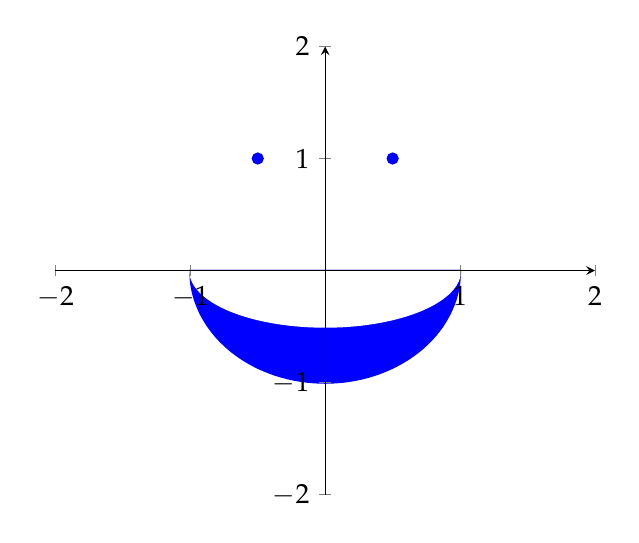
\begin{tikzpicture}
      \begin{axis}[ axis x line=middle, axis y line=middle,
        xmax=2, xmin=-2,
        ymax=2, ymin=-2,
        area style]
        \addplot[thick, color=blue, smooth, domain=-pi:0,fill,blue] ({cos(deg(\x))},{sin(deg(\x))}) \closedcycle;
        \addplot[thick, color=blue, smooth, domain=-pi:0,fill,white] ({cos(deg(\x))},{0.5*sin(deg(\x))}) \closedcycle;
        \addplot[only marks, mark=*, blue] coordinates {
          (0.5, 1)
          (-0.5, 1)
        };
      \end{axis}
    \end{tikzpicture}
  \end{center}

\end{example}

\begin{definition}
  If $A$ and $B$ are sets with $A \cap B = \emptyset$, we say that $A$ and $B$ are \emph{disjoint}.
\end{definition}
Informally, disjoint means that the sets have no elements in common.

%%% Local Variables:
%%% TeX-master: "Proofs"
%%% End:
\probsec{~\ref{sec:prod-union-inters}}
\begin{enumerate}
  \item Suppose $A$ and $B$ are sets. Prove that $A \cap B \subset A \cup B$.

  \item Suppose that $A$ and $B$ are sets, and that $A \cap B = A \cup B$. What can you conclude?\sidenote{If you're thinking, ``How the heck should I know?'', then I highly recommend doing out several examples. That is, choose different pairs of sets $A$ and $B$, and test to see if the equality $A \cap B = A \cup B$ holds or not. Then try to see if there is a pattern to the cases where equality does hold.} Prove your answer.
\end{enumerate}



\section{Complements and set difference}
\label{sec:compl-set-diff}

\begin{definition}
  If $A$ and $B$ are sets, then the \emph{set difference} $A - B$ is \marginnote{Some texts use the notation $A \setminus B$.}
  \[
  \{x \mid x \in A \text{ and } x \notin B\}.
  \]
\end{definition}
This means we start with everything in $A$, but then throw out all of those things which happen to be in $B$.

\begin{example}
  Let $A = \{$chocolate, strawberries, mold, cake, garbage, dirt, ice cream$\}$ and $B = \{\text{mold, garbage, dirt}\}$. Then $A - B$ should be the set consisting of only the yummy things from $A$.
\end{example}

\begin{example}
  Let $A = \{1, 2, 3\}$, $B = \{3\}$, $C = \{3, 4, 5\}$, and $D = \emptyset$. Then
  \begin{itemize}
      \item $A - B = \{1, 2\}$,
      \item $A - C = \{1, 2\}$, and
      \item $A - D = \{1, 2, 3\}$.
  \end{itemize}
  Notice that in $A - C$, the elements $4$ and $5$ play no role! Neither is in $A$ to begin with, and so we never have to throw them out.
\end{example}

\subsection{The universe}
\label{sec:universe}

To define the even numbers, one could say
\[
\{n \in \Z  \mid  n \text{ is even}\}
\]
but frequently one just writes
\[
\{n  \mid  n \text{ is even}\}.
\]
Similarly, in calculus, variables almost always represent real numbers, but this is rarely explicitly stated. More generally, the set where most of our basic objects come from in any given context is called the \emph{universe}; in calculus, the universe would be $\R$, and in the even numbers example, the universe would be $\Z$. If the universe is understood, then it is often omitted from the set-builder notation, as in the even numbers example above. Thus, if our universe is the set $U$, then we interpret
\[
\{x  \mid  P(x)\} 
\]\marginnote{Here, $P(x)$ is the open statement P applied to $x$.}
to mean
\[
\{x \in U  \mid  P(x)\}.
\]
If there is any doubt about what the universe is, then the second form should be used. Note that if $A$ is a set with universe $U$, then automatically $A \subset U$.

\begin{definition}
  Let $A$ be a set with universe $U$. Then the \emph{complement} of $A$ is $U - A$. It is written $A^c$, which is read ``$A$ complement''.
\end{definition}

If $E$ is the set of even integers, then we usually take $U = \Z$, from which $E^c$ is the set of odd integers. What if $A = \{0\}$? What is $A^c$? In this case, it's not at all obvious what the universe is. If the universe is $\Z$, then $A$ is the set of nonzero integers. But what if the universe is $\R$, or $\C$?

Now suppose that 
\[
U = \{\text{Judgments you can make about your neighbor's clothes}\}.
\]
Let $A \subset U$ consist of the set of insults. Then the complement of $A$ is the set of compliments!\sidenote{I suppose there are also neutral comments, but this just ruins the joke.}

\begin{proposition}\label{prop:complements}
  Let $A$ be a set with universe $U$. Then
  \begin{enumerate}[(a)]
      \item $A \cap A^c = \emptyset$.
      \item $A \cup A^c = U$.
      \item $(A^c)^c = A$.
      \item $\emptyset^c = U$.
      \item $U^c = \emptyset$.
  \end{enumerate}
\end{proposition}

The proof is left as an exercise.

%%% Local Variables:
%%% TeX-master: "Proofs"
%%% End:
\probsec{~\ref{sec:compl-set-diff}}
\begin{enumerate}
    \item Let $A = \Z$, $B = \{n \in \Z \mid n \text{ is even}\}$, $C = \{0\}$, and $D = \{x \in \R \mid x <0\}$. For all of the following, make sure to prove your answer.
  \begin{enumerate}
      \item What is $A - B$?
      \item What is $B - A$?
      \item What is $A - (B - C)$?
      \item What is $A - D$?
      \item What is $(A \cap B) - (C \cup D)$?
  \end{enumerate}

    \item Prove that $A - B = A \cap B^c$.

    \item Prove that $(A \cup B) - (A \cap B) = (A - B) \cup (B - A)$.\sidenote{The expressions on both sides of the equation are often called the \emph{symmetric difference} of $A$ and $B$, written $A \triangle B$.}

    \item Prove that $(A \cap B) \cup (A \cap B^c) = A$.
\end{enumerate}


\section{Power set}
\label{sec:power-set}

\begin{definition}
  Let $S$ be a set. The \emph{power set} of $S$, written $\sP(S)$, \marginnote{Some texts use the notation $2^S$ for the power set. There is a more general notation $B^A$, which means the set of functions from $A$ to $B$.} is the set of all subsets of $S$.
\end{definition}
If $S = \emptyset$, then $\sP(S) = \{\emptyset\}$. Note that $S \neq \sP(S)$---while $S$ is the empty set, $\sP(S)$ is the set containing the empty set. To see the difference, observe that $\# S = 0$ but $\# \sP(S) = 1$.

If $S \neq \emptyset$, then $\sP(S)$ always contains the two elements $\emptyset$ and $S$ itself. Here are some simple examples:
\begin{itemize}
    \item If $S = \{a\}$, then $\sP(S) = \{\emptyset, \{a\}\}$.
    \item If $S = \{a, b\}$, then $\sP(S) = \{\emptyset, \{a\}, \{b\}, \{a, b\}\}$. Note that $a \notin \sP(S)$; rather, $\{a\} \in \sP(S)$.
    \item If $S = \{a, b, c\}$, then $\sP(S)$ is
  \[
  \begin{array}{cccc}
    \{\emptyset, & \{a\}, & \{b\}, & \{a, b\}, \\
    \{c\}, & \{a, c\}, & \{b, c\}, & \{a, b, c\}\}.
  \end{array}
  \]
\end{itemize}
It can be useful to relate the subsets to each other graphically. Take the example of $S = \{a, b, c\}$. \marginnote[.5in]{The astute reader will notice that the diagram looks like a perspective drawing of a cube. This is not a coincidence! Compare, for example, opposite faces of the cube. What do you observe?}
\[
\xymatrix{
  & \{a, b, c\} \ar@{-}[dl] \ar@{-}[d] \ar@{-}[dr] & \\
  \{a, b\} \ar@{-}[d] \ar@{-}[dr] & \{a, c\} \ar@{-}[dl] \ar@{-}[dr] & \{b, c\} \ar@{-}[dl] \ar@{-}[d]\\
  \{a\} \ar@{-}[dr] & \{b\} \ar@{-}[d] & \{c\} \ar@{-}[dl] \\
  & \emptyset &
}
\]
In the diagram, if two sets are connected by a line, then the lower set is a subset of the upper set.

\begin{proposition}
  Suppose $S$ is a finite set. Then $\# \sP(S) = 2^{\# S}$.
\end{proposition}

\begin{proof}
  Suppose $\# S = n$, and $S = \{x_1, x_2, \dots, x_n\}$. Given a subset $X \subset S$, we ask $n$ questions about it: is $x_1$ in $X$, is $x_2$ in $X$, \dots, is $x_n$ in $X$? Notice that the answers to these questions uniquely determines $X$.\sidenote{``Uniquely determines'' means that knowing the answers to these questions is identical to knowing $X$ itself. Note that if all the answers are ``no'', then $X = \emptyset$.} As each question has exactly two possible answers, there are $2 \cdot 2 \cdot \cdots \cdot 2 = 2^n$ possible sequences of answers to all $n$ questions. Therefore, there are exactly $2^n$ possible subsets $X$.
\end{proof}

%%% Local Variables:
%%% TeX-master: "Proofs"
%%% End:
\probsec{~\ref{sec:power-set}}
\begin{enumerate}
    \item Suppose $A = \{1, 2\}$, $B = \{b,c\}$, and $C = \{(1,c), (2,b)\}$. Write the following sets in list form.
  \begin{enumerate}
      \item $\sP(A)$
      \item $\sP(C)$
      \item $\sP((A \times B) - C)$
      \item $\sP(\sP(\emptyset))$.
  \end{enumerate}

    \item True or false: if $A \subset B$, then $\sP(A) \subset \sP(B)$.\sidenote{You should of course prove your answer. If false, it's enough to come up with a single example.}

    \item Prove that $A = B$ if and only if $\sP(A) = \sP(B)$.

    \item Let $S = [0,6] \times [0,2]$. A powerful eccentric alien orders every adult on the planet to choose an element of $\sP(S)$. If any two people choose the same element, the planet will be vaporized. Otherwise, we each get a bag of cherries. What element would you choose? Is there some easy instruction that you could give humanity to guarantee survival?
\end{enumerate}


\section{Indexed sets}
\label{sec:indexed-sets}

Suppose we have a bunch of different sets we want to study. If there are three, we could name them $A$, $B$, and $C$ (for example). What if there are 10? One could conceivably call them $A$, $B$, $C$, \dots, up until the 10th letter of the alphabet, which off the top of my head is \dots well, whatever it is! But of course it's easier to name them, for example, $A_1$, $A_2$, \dots, $A_{10}$. The subscripts are often called \emph{indices}, or in the singular an \emph{index}. In this case, the indices are $n \in \N, 1 \leq n \leq 10$, or more simply $n = 1, 2, \dots, 10$.

But this is mathematics! Why stop at $10$? Let's take the following example. A real-valued function $f(x)$ is said to be \emph{bounded} if there exists some real number $L$ such that $|f(x)|$ never exceeds $L$. Any constant function is bounded, as are $\sin x$, $\cos x$, and $e^{-x^2}$. The function $f(x) = x$ is \emph{not} bounded, as $\lim_{x \to \infty} f = \infty$.

Given $M \in \N$, let 
\[
F_M = \{f(x) \mid f \text{ is a real-valued function and } |f(x)| \leq M \text{ for every } x\}.
\]
For example, $3\sin x \in F_3$, but $3\sin x \notin F_2$. Put another way, $F_2$ consists of functions whose graphs lie entirely between the lines $y = 2$ and $y = -2$. Let $B = $ the set of all bounded functions. In other words,
\[
B = \{f(x) \mid f \text{ is a real-valued function and } \exists L \in \R \text{ such that } |f(x)| \leq L \, \, \forall x\}.
\]

\begin{claim}
  With $B$ and $F_M$ as above, $B = \displaystyle\bigcup_{M \in \N} F_M$. \marginnote{The union notation is the same as $F_1 \cup F_2 \cup \cdots$.}
\end{claim}
Notice that we're taking the union of infinitely many sets! The definition is the same as for two sets: $f \in \bigcup F_M$ means $f$ is in one of the $F_M$s, and vice versa.

The idea of the proof is that in order for a function to be bounded, it is in fact bounded by some integer $M$. But this means that the function is in $F_M$ for that particular value of $M$. \marginnote{Note that we need \emph{all} of the $F_M$, since $N \sin x \notin F_M$ whenever $N > M$.}

\begin{proof}
  We need to show that $\bigcup_{M \in \N} F_M \subset B$ and that $B \subset \bigcup_{M \in \N} F_M$. For the first containment, suppose $f(x) \in \bigcup F_M$. By definition of union, this means that $f(x)$ is in one of the $F_M$, say $F_{M_0}$. \marginnote{Notice that in order to write this proof, you need to know lots of definitions, and know them precisely!} By definition of $F_{M_0}$, this means that $|f(x)| \leq M_0$ for all $x$. By definition of bounded, we see that $f(x)$ is bounded. Therefore $f(x) \in B$, and so $\bigcup F_M \subset B$.

  Now suppose $f(x) \in B$. This means that $f(x)$ is bounded. By definition of bounded, \marginnote{Look, more definitions!} there exists some $L \in \R$ such that $|f(x)| \leq L$ for all $x$. Let $M_0$ be any integer larger than $L$---for example, $M_0 = \lfloor L + 1\rfloor$.\sidenote{The function $\lfloor x \rfloor$ is the \emph{greatest integer function}, which means essentially write the number as a decimal and then drop everything after the decimal point.} Then we see see that $|f(x)| \leq M_0$ as well. Therefore $f(x) \in F_{M_0}$ by definition of $F_{M_0}$, and we obtain $f(x) \in \bigcup_{M \in \N} F_M$ by definition of union. We conclude that $B \subset \bigcup_{M \in \N} F_M$.

  Since $\bigcup_{M \in \N} F_M \subset B$ and $B \subset \bigcup_{M \in \N} F_M$, we see that $B = \bigcup F_M$.
\end{proof}

So what just happened? We found a way to write the set of bounded functions as a union of a bunch of other sets---in fact, of infinitely many sets. We refer to each of these sets with a positive integer. In other words, our indices are exactly the elements of $\N$. The way this is usually phrased is, $\N$ is the \emph{index set} for the $F_M$. 

In general, the indices don't even have to be integers.
\begin{example}
  Let $C = \{\text{people in this class}\}$. For $c \in C$, let $L_c$ be the set of letters in $c$'s full name. Then $\displaystyle\bigcap_{c \in C} L_c$ is the set of letters which every person's name contains. This set is \emph{probably} empty---well, that's my wild guess. In this case, the index set is $C$.
\end{example}

For clarity, let us rigorously define the intersection and union of an arbitrary collection\sidenote{As opposed to just two.} of sets.
\begin{definition}
  Let $\Lambda$ be an index set, and for each $\lambda \in \Lambda$ let $A_\lambda$ be a set. Then
  \[
  \bigcup_{\lambda \in \Lambda} A_\lambda
  \]
  is the set consisting of all $x$ such that $x$ is contained in at least one of the $A_\lambda$. Also,
  \[
  \bigcap_{\lambda \in \Lambda} A_\lambda
  \]
  is the set consisting of all $x$ such that $x$ is contained in every $A_\lambda$.
\end{definition}
Here is an example. Let $\Lambda = \R$, and define $A_\lambda$ to be the set $\{\lambda\}$. So $A_0 = \{0\}$, $A_\pi = \{\pi\}$, and so forth. Then
\[
\bigcup_{\lambda \in \R} A_\lambda = \R
\]
and
\[
\bigcup_{\lambda \in \Q} A_\lambda = \Q.
\]

%%% Local Variables:
%%% TeX-master: "Proofs"
%%% End:
\probsec{~\ref{sec:indexed-sets}}
\begin{enumerate}
    \item For $i \in \N$, let $A_i = \{-i, -i+1, \dots, i-1, i\}$.
  \begin{enumerate}
      \item Write $A_i$ in set-builder notation.
      \item What is $A_1 \cup A_2 \cup A_3$?
      \item What is $A_1 \cup A_2 \cup \cdots \cup A_{n}$?
      \item What is $\displaystyle\bigcup_{i \in \N} A_i$?
      \item What is $\displaystyle\bigcap_{i\in\N} A_i$?
  \end{enumerate}

    \item Let $I_n = (\frac{1}{n}, 1]$. (This is interval notation.) What is $\displaystyle\bigcup_{n \in \N} I_n$? You do not need to prove your answer.

    \item For $n \in \N$, let $A_n$ be the interval $(-\frac{1}{n}, \frac{1}{n})$. What are $\cup A_n$ and $\cap A_n$?\sidenote{The omission of the index means over all possible $n$. This is analogous to writing, for example, $\sum a_n$ instead of $\displaystyle\sum_{n=1}^{\infty} a_n$.} You do not need to prove your answer.

    \item Let $A_y \subset \R^2$ where $y \in \R$ be given by $A_y = \{(x, x+y): x \in \R\}$. You do not need to prove your answers.
  \begin{enumerate}
      \item Graph $A_1 \cup A_2 \cup A_3$.
      \item Graph $\displaystyle\bigcup_{y \in \Z} A_y$.
      \item Graph $\displaystyle\bigcup_{y \in \N} A_y$.
      \item Graph $\displaystyle\bigcup_{y \in \R} A_y$.
      \item Graph $\displaystyle\bigcup_{y \geq 0} A_y$.
  \end{enumerate}

    \item Let $B_x \subset \R^2$ where $x \in \R$ be given by $B_x = \{(x, x+y): y \in \R\}$. You do not need to prove your answers.
  \begin{enumerate}
      \item Graph $B_1 \cup B_2 \cup B_3$.
      \item Graph $\displaystyle\bigcup_{x \in \Z} B_x$.
      \item Graph $\displaystyle\bigcup_{x\in \N} B_x$.
      \item Graph $\displaystyle\bigcup_{x \in \R} B_x$.
      \item Graph $\displaystyle\bigcup_{x \geq 0} B_x$.
  \end{enumerate}

    \item For $n \in \Z$, let $A_n \subset \Z$ be the set of multiples of $n$. What are $\cup A_n$ and $\cap A_n$?

    \item Let $A_\alpha = \{(x,y): |y| \leq x^2/\alpha\}$ where $\alpha \in \R$ and $\alpha > 0$. Graph $\cap A_\alpha$ and $\cup A_\alpha$.

    \item Suppose $A_i \subset \cap A_j$ for every $i$. What can you conclude?

    \item Suppose $\cup A_j \subset A_i$ for every $i$. What can you conclude?

    \item Let $A$ be a set. \marginnote{This problem does not properly speaking feature \emph{indexed} sets, but it does refer to a union and intersection of a collection of sets.}
  \begin{enumerate}
      \item Compute $\displaystyle\bigcup_{X \in \sP(A)} X$. 
      \item Compute $\displaystyle\bigcap_{X \in \sP(A)} X$.
  \end{enumerate}


    \item For $(r, n) \in \Q \times \N$, let $A_{(r,n)}$ be the interval $(r - \frac{1}{n}, r + \frac{1}{n})$. Compute the following. You do not need to prove your answers.
  \begin{enumerate}
      \item $\displaystyle\bigcap_{r \in \Q} \bigcup_{n \in \N} A_{(r,n)}$
      \item $\displaystyle\bigcup_{r \in \Q} \bigcap_{n \in \N} A_{(r,n)}$
      \item $\displaystyle\bigcup_{n \in \N} \bigcap_{r \in \Q} A_{(r,n)}$
      \item $\displaystyle\bigcap_{n \in \N} \bigcup_{r \in \Q} A_{(r,n)}$
  \end{enumerate}

\end{enumerate}



\bibliographystyle{halpha}
\end{document}